% IFAC International Federation of Automatic Control paper template. 
% Created by: ?
% Modified by: Rasmus Christensen, Aalborg University, Denmark 15/12/2012
\documentclass{ifacconf}

\usepackage{natbib}            % you should have natbib.sty
\usepackage{graphicx}          % Include this line if your 
                               % document contains figures,
%\usepackage[dvips]{epsfig}    % or this line, depending on which
                               % you prefer.
\usepackage[utf8]{inputenc} % So we can input Nicks name in the paper title!
\usepackage[T1]{fontenc}
\usepackage{amsmath,amsfonts,amssymb} % Added so we can do pretty math equations.

% predefined environments
%\begin{thm} ... \end{thm}		% Theorem
%\begin{lem} ... \end{lem}		% Lemma
%\begin{claim} ... \end{claim}	% Claim
%\begin{conj} ... \end{conj}	% Conjecture
%\begin{cor} ... \end{cor}		% Corollary
%\begin{fact} ... \end{fact}	% Fact
%\begin{hypo} ... \end{hypo}	% Hypothesis
%\begin{prop} ... \end{prop}	% Proposition
%\begin{crit} ... \end{crit}	% Criterion


\begin{document}

\begin{frontmatter}

\title{Centralized State Estimation of Distributed Maritime Autonomous Surface Oceanographers\thanksref{footnoteinfo}} % Title, preferably not more than 10 words.

\thanks[footnoteinfo]{The prototype of AAUSHIP.01 and all components has been paid for in full by the School of Information Communication and Technology, Aalborg University.}

\author{Rasmus L. Christensen,} 
\author{Frederik Juul,} 
\author{Nick \O stergaard,}
\author{Jesper A. Larsen}
\address{Section of Automation and Control, Department of Electronic Systems, Aalborg University, Fredrik Bajers Vej 7, 9220 Aalborg \O st, Denmark (e-mail: \{ralch,nickoe,fjuul,jal\}@es.aau.dk)}                                            
          
\begin{keyword}                           % Five to ten keywords,  
Centralized control; baud rates; state estimation; marine systems; master slave system.              % chosen from the IFAC 
\end{keyword}                             % keyword list or with the 
                                          % help of the Automatica 
                                          % keyword wizard


\begin{abstract}                          % Abstract of not more than 250 words.
This paper considers the subject of running a centralized controller for the purpose of navigating a small Autonomous Surface Vehicle (ASV). The centralized controller is using a Kalman filter as a state predictor to improve the precision of the navigational aids mounted aboard. This work presents the design of the motion control system as well as an estimator designed to cope with packet losses. 
\end{abstract}

\end{frontmatter}

\section{Introduction}
Seaborne measurements are often an expensive and time-consuming task. They could however in many cases have a large impact on the area where they are obtained. At the Fukushima accident in 2011 the area of effect in the water and the safety margin was primarily based on estimates, as only few measurements were available. \cite{energy}.
The coastal areas around Greenland are another area which could benefit from seaborne measurements as up to date maps are not available. This causes the ships which need to pass near the coast to have a higher safety margin, which in turn lowers the amounts of traffic possible. If a ship would need to get very close to the shores, up to date maps of the area would also be a requirement. This need is acknowledged and is considered important for the flourishing greenlandic industrialization by the government of Denmark, but the project does not have sufficient funding. \cite{engineer}.

One way to reduce the cost of such maritime measurements would be to develop small autonomous drones to carry out the task. These should be controlled by a mothership to enable easy scalability and coordination. Further, they should communicate using a simple data link to preserve bandwidth and limit power consumption. The system should be robust to dataloss and measurementnoise which can be expected from low cost sensors. This can be achieved through sensor fusion.

Currently the main focus of autonomous vehicles have been on aerial, ground and underwater vehicles, while there is close to no research going on about small autonomous surface vessels. An example of such a vessel is the Stingray ASV developed by Isreali based Elbit Systems. 
\begin{figure}
	\begin{center}
		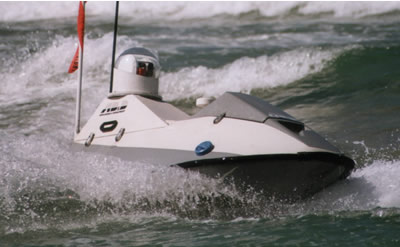
\includegraphics[width=8.4cm]{img/stingray.jpg} % width of a column is 8.4 cm.
		\caption{The autonomous surface vehicle Stingray by Israeli based Elbit Systems in action \cite{defense}.}  
		\label{fig:stingray}
	\end{center}
\end{figure}

Figure \ref{fig:stingray} depicts the Stingray. It is primarily developed as an aid in the battle agains pirates and for SAR (search and rescue) missions, but can also be equipped with other sensory equipment, which can be used to map the sea bed, or measure the amount of radiation in coastal areas. 

The scope of this project is however to develop a smaller vehicle, which in turn could function as part of a measuring swarm, controlled by a mother ship, thus making measuring missions more efficient and less time consuming. As the price of such a swarm system for measurement purposes would be high if systems like the Stingray is to be used, the suggestion of this project, is to develop a small cost-efficient vessel. Throughout this project, a prototype vessel AAUSHIP.01 have been developed, taking into account the hull design, choosing electronics and so forth. This paper will only describe the development of the estimation and control algorithms. Figure \ref{fig:ship} depicts the prototype used in the project. This ship is fitted with two 1200W engines which are run as a differential system (making it a ship without rudders), making the ship turn by reducing the input on one engine and reducing it on the other, and vice-versa. 

\begin{figure}
	\begin{center}
		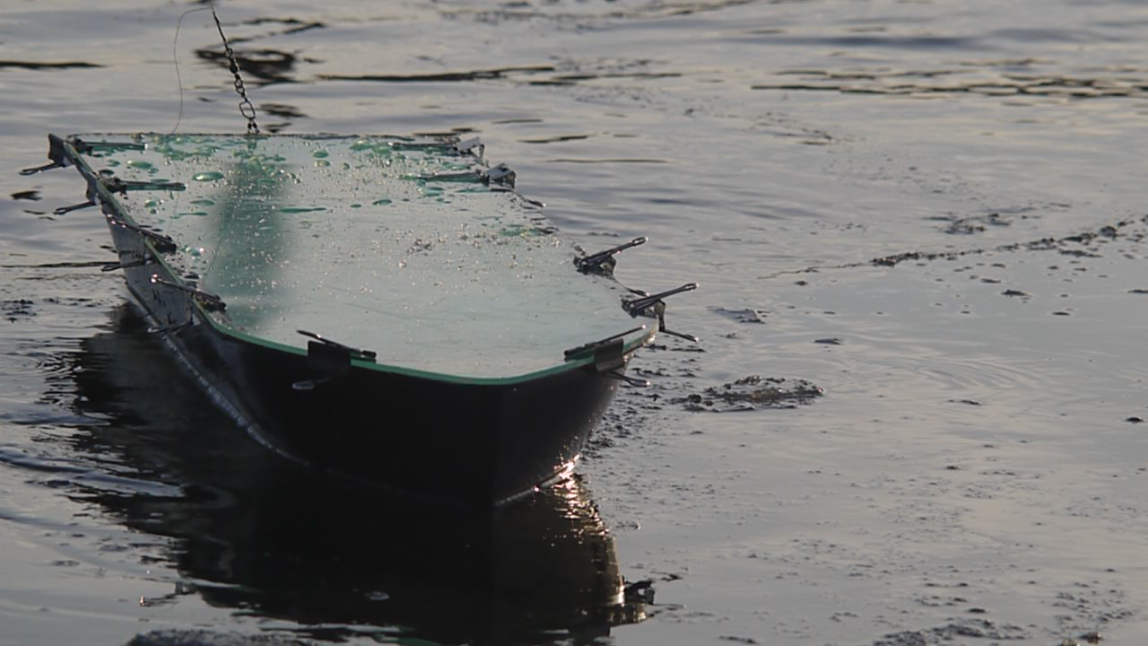
\includegraphics[width=8.4cm]{img/aauship.png} % width of a column is 8.4 cm.
		\caption{AAUSHIP.01 - a prototype of an autonomous maritime surface oceanographer, as this is only a prototype, the lid is held in place with clamps. }  
		\label{fig:ship}
	\end{center}
\end{figure}

\subsection{Problem statement}
Is it possible to develop a centralized state estimator for use in the maritime environment using a small data link?

\section{Methods}

This project is primarily based around the linearized state space model derived for the ship, which are then utilized as 

\subsection{Modeling of the ship}

AAUSHIP.01 is designed as a non-planing displacement ship, which are not to sail in any form of rough sea, which makes for the simplification of the vessel being modeled as a 3 DOF vessel, with the states given as $(x,y,\theta)$, describing the motion in the x direction, the motion in y and the yaw angle about the z-axis. From this, the model is derived using the formula described in \cite{cyber} which gives the following model:
\begin{align}
\dot{\vec{x}} = \begin{bmatrix}
-\beta_{\dot{x}} & 0 & 0\\
0 & 0 & 1\\
0 & 0 & -\beta_{\omega} \end{bmatrix}\begin{bmatrix}
\dot{x}\\
\theta\\
\omega
\end{bmatrix} + \begin{bmatrix}
m^{-1} & 0\\
0 & 0\\
0 & m^{-1}
\end{bmatrix}\begin{bmatrix}
F\\
\tau
\end{bmatrix}
\label{eq:sscont}
\end{align}
Where $\beta$ denotes the skin frictional drag divided by the mass $m$. This equation is a simplified version of the entire system, where the effects of damping, coriolis and the like have not been accounted for. This simplification is fair as AAUSHIP.01 is relatively small, and the areas it is built to map are small as well. For the purpose of controlling the vessel, a simple LQR feedback controller have been implemented alongside a reference gain, these are described in (\ref{eq:fcont}) and (\ref{eq:ncont}). The system is implemented on the on-board controller, and is digitized using the zero-order hold theorem. This gives converts the system to as in (\ref{eq:digit}). 
\begin{align}
\vec{x}[k+1] = \begin{bmatrix}
-\beta_{\dot{x}} & 0 & 0\\
0 & 1 & 1\\
0 & 0 & -\beta_{\omega} \end{bmatrix}\begin{bmatrix}
\dot{x}[k]\\
\theta[k]\\
\omega[k]
\end{bmatrix} + \begin{bmatrix}
m^{-1} & 0\\
0 & 0\\
0 & m^{-1}
\end{bmatrix}\begin{bmatrix}
F[k]\\
\tau[k]
\end{bmatrix}
\label{eq:digit}
\end{align}
\textbf{indsæt rigtig formel!}

\subsection{Navigation}

The navigation controller of the ship is a reference heading calculator, which outputs the required direction of movement to reach the next waypoint. In order to efficiently and accurately navigate along the path, a set of sub-waypoints is calculated for each route between two Waypoints. The main control strategy is to navigate through all of these SWPs in a predefined order, one by one. The heading of the ship is defined in NED\footnote[1]{[North, East, Down]} coordinate system. The required heading is determined based on the position of the ship and the position of the next sub-waypoint.

\subsection{State estimation}
To give a better estimate of position and the attitude of the craft, a Kalman filter have been implemented to improve the accuracy of the sensors mounted aboard the ship. To develop a such, the discrete time state model of the ship have been derived to be:
\begin{align}
\vec{\Phi} = diag\{\vec{\Phi} _x,\vec{\Phi} _y,\vec{\Phi} _\omega\}
\end{align}
Where the diagonal entries $\vec{\Phi} _x,\vec{\Phi} _y,\vec{\Phi} _\omega$ are given by the same equation, with different entries:
\begin{align}
\vec{\Phi}_{x,y,\omega}(k) = \begin{bmatrix}
1 & t_s & 0\\
0 & 1 & t_s\\
0 & -\beta_{x,y,\omega} & 0
\end{bmatrix}
\label{eq:kal}
\end{align}
In equation (\ref{eq:kal}), $\beta_{x,y,\omega}$ denotes the skin frictional acceleration drag in the $x$,$y$ and $\omega$ direction respectively, $m$ is the mass of the craft, $I$ is the inertia and $t_s$ is the sampling time of the filter. The acceleration of the craft $\ddot{x}$,$\ddot{y}$ and $\alpha$ are omitted as the error grows exponentially which have produced bad results. The states to be estimated for the controller are:
\begin{align}
^b\hat{\vec{x}_k} = \begin{bmatrix}
x & \dot{x} & y & \dot{y} & \theta & \omega
\end{bmatrix}^T
\end{align}
The observation model of the filter does however contain more measurements, and the measurements are given as:
\begin{align}
\vec{v}_k = \begin{bmatrix}
x & \dot{x} & \ddot{x} & y & \dot{y} & \ddot{y} & \theta & \omega & \alpha
\end{bmatrix}^T
\end{align}
To tune the filter the covariance matrices $\vec{R}_k$ and $\vec{Q}_k$ are a function of the measurement distribution and the input distribution. The input to the system is given as:
\begin{align}
\vec{w}_k = \vec{B}\vec{u}
\end{align}
Where $\vec{B}$ is an augmented version of the system input matrix defined in (\ref{eq:ss_cont}) and $\vec{u}$ is the inputs to the system given as a force $F$ and a torque $\tau$. $\vec{B}$ is given as 
\begin{align}
\vec{B} = \begin{bmatrix}
0 & 0 & \frac{1}{m} & 0 & 0 & 0 & 0 & 0 & 0\\
0 & 0 & 0 & 0 & 0 & 0 & 0 & 0 & \frac{1}{I} \end{bmatrix}^T
\end{align} 
And the input is given as $\vec{u} = \begin{bmatrix}F\ & \tau\end{bmatrix}^T$. As $\vec{B}$ is a static matrix, it is only the distribution of the force $F$ and the torque $\tau$ that is of interest. The distribution of the force affecting the ship can be split into an $x$- and $y$-component, as the ship is also expected to move slightly sideways. The distributions of the force is given as white Guassian noise processes, thus stating:
\begin{align}
F&\sim \mathcal{N}(\vec{\mu}_F,\vec{\sigma}^2_F)\\
\tau&\sim \mathcal{N}(\mu_\tau,\sigma^2_\tau)
\end{align}
Where the tuning through simulations have yielded the best results using $\vec{\mu}_F = \begin{bmatrix}5.4355 & 0\end{bmatrix}^T$. The first entry is because to the ship is for most of the time moving along at 1 m/s and that is the estimated force required to thrust the ship forward at 1 m/s with the frictional drag the ship experiences. The latter is the force in the $y$-direction which is given as a zero-mean process as the ship generally is expected not to move sideways. The torque is also given as a zero-mean process as the ship for most of the time is moving straight. The covariance matrix for the input, can thus be given as the covariance of $\vec{B}\vec{u}$ which gives the following:
\begin{align}
\vec{R}_k = \text{diag}\{0,0,\sigma^2_{F(1,1)},0,0,\sigma^2_{F(2,1)},0,0,\sigma^2_\tau\}
\end{align}
The measurement covariance is more interesting, as this contains the actual variance of the measurements, and play a big part in how much each of these are weighted in Kalman gain $\bar{\vec{K}}$. Static tests have been conducted to estimate these variances, and all the sensors are assumed to be Gaussian white noise processes, thus defining:
\begin{align}
\vec{v}_k  \sim \mathcal{N}(\vec{\mu}_v,\vec{\sigma}^2_{v})
\end{align}
As all the measurements are independent, the covariance matrix is given as:
\begin{align}
\vec{Q}_k = \text{diag}\{\vec{\sigma}^2_{v}\}
\end{align}
Where $\vec{\sigma}^2_{v} = \begin{bmatrix}\sigma^2_x & \sigma^2_{\dot{x}} & \sigma^2_{{\ddot{x}}} & \sigma^2_y & \sigma^2_{\dot{y}} & \sigma^2_{{\ddot{y}}} & \sigma^2_\theta & \sigma^2_\omega & \sigma^2_\alpha \end{bmatrix}^T$. As the velocity output of the GPS device $\dot{x}$ is an absolute value, the estimate of this is a bit different as the distribution when still is not equal to the distribution when moving. To estimate the variance of $\dot{x}$ the unbiased sample variance formula is used, which computes the variance, even though the samples only consist of absolute values. 

The actual implementation of the filter is an altered version of an Linear Minimum Mean Square Error filter - the alteration lies in the Kalman gain, where a matrix mask $\vec{\Lambda}$ is post multiplied. This matrix mask is to zero out the measurements that are invalid. This matrix mask is defined as:
\begin{align}
\vec{\Lambda} = diag\{ \lambda_x,\lambda_{\dot{x}},\lambda_{\ddot{x}},\lambda_y,\lambda_{\dot{y}},\lambda_{\ddot{y}},\lambda_{\theta},\lambda_{\omega},\lambda_{\alpha} \}
\end{align}
This ensures that when a measurement is invalid (the checksum is not true) the receiver zeros out the gain, and runs the filter on the other sensors / estimates. The individual $\lambda$s are thus given as:
\begin{align}
\lambda = 
\left\{
  \begin{array}{l l}
    1 & \quad \text{if checksum is valid}\\
    0 & \quad \text{otherwise}
  \end{array} \right.
\end{align} 
This makes sure to zero out the Kalman gain $\bar{\vec{K}}$ if a packet is corrupted instead of making the filter run on faulty data. When this is implemented, the system handles packet loss by making the filter run on estimates for the next sample, rather than running on a faulty measurement.

\subsection{Modelling and Controls}
The model of the ASV is in continuos time given as the state space equation defined in (\ref{eq:sscont}) - the model considers the motion of the ship with 3 degrees of freedom, movement in the $x$-direction, $y$-direction and rotation about the z-axis $\omega$. This reduced model is sufficient as it is only the velocity and the angle that is control variables. The control strategy for this project is to track the input reference, and use an optimal feedback gain to reach the desired values. This is done as in \cite{feedback} resulting in the following gains:
\begin{align}
F_{opt} &= \begin{bmatrix}
15.1668 & 0 & 0\\
0 & 2.5165 & 0.7134
\end{bmatrix}\label{eq:fcont}\\
N &=  \begin{bmatrix}
24.0668 & 0\\
0 & 2.5165
\end{bmatrix}\label{eq:ncont}
\end{align}
For implementation purposes the system is discretized using the MATLAB command \texttt{c2d} with a samping time of $t_s = \frac{1}{3}$, and then using the same algorithms as in equation (\ref{eq:fcont}) and (\ref{eq:ncont}) for computing the optimal feedback and reference gain respectively, thus resulting in the gains (\ref{eq:fdisc}) and (\ref{eq:ndisc}):
\begin{align}
_\mathcal{D}F_{opt} &= \begin{bmatrix}
10.6956 & 0 & 0\\
0 & 2.2743 & 0.6681
\end{bmatrix}\label{eq:fdisc}\\
_\mathcal{D}N &=  \begin{bmatrix}
19.5956 & 0\\
0 & 2.2743
\end{bmatrix}\label{eq:ndisc}
\end{align}
As the controller outputs a desired force $F$ and a torque $\tau$ dependent on the reference angle $\theta$ and velocity $\dot{x}$. This output must be converted to a set-point number of revolutions, as this is the input to the low-level system handling the engines. The force of the forward motion of the ship is given as a function of the number of revolutions of the propeller $n$, this relation is defined by \cite{cyber} to be as in (\ref{eq:soren}):
\begin{align}
F = \rho \cdot D^4 \cdot K_T \cdot |n| \cdot n
\label{eq:soren}
\end{align}
As the two engines both produce both a force and a torque, as a function of the same revolutions, the matrix equation $\vec{x} = \vec{A}^{-1}\vec{b}$ can be solved for the number of revolutions the engines need to produce as in (\ref{eq:solver}):
\begin{align}
\begin{bmatrix}
n_1^2\\
n_2^2
\end{bmatrix} = \begin{bmatrix}
C_1 & C_1\\
C_1 \cdot l \cdot \sin(\theta_\text{stbd.}) & C_1 \cdot l \cdot \sin(\theta_\text{port})
\end{bmatrix}^{-1}\begin{bmatrix}
F_\text{desired}\\
\tau_\text{desired}
\end{bmatrix}\label{eq:solver}
\end{align}
The revolutions of the propeller can assume negative values (if the ship is reversing), so what is left to do now, is to solve for $n_1$ and $n_2$. These can be solved by rearranging (\ref{eq:solver}):
\begin{align}
n_{port-setpoint} = \text{sign}(n_1^2) \cdot \sqrt{n_1^2}\\
n_{stbd-setpoint} = \text{sign}(n_2^2) \cdot \sqrt{n_2^2}
\end{align}
Thus giving the engine set-points as a function of the forces of the system.

\subsection{Controller verification}
To verify wether the system actually works, two tests have been conducted in a small lake at the Aalborg University campus area. The goal of the test, was to verify that the theory used in developing AAUSHIP.01 actually worked. The test was performed in calm water, and the ship was programmed to follow a path.  
\begin{figure}
	\begin{center}
		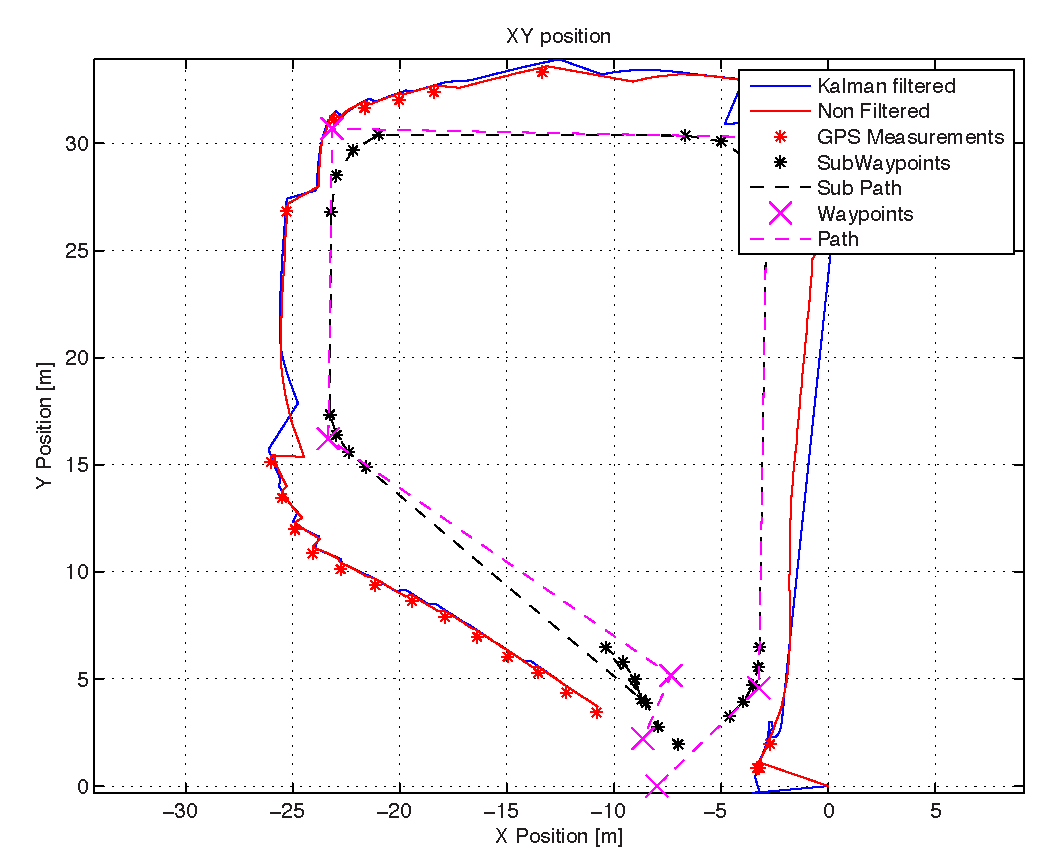
\includegraphics[width=8.4cm]{img/position}    % The printed column  
		\caption{Test 1 of the control and position estimation. The test is performed in the Klingenberg Pond at Aalborg University.}
		\label{fig:position}               
	\end{center}                                 % accordingly.
\end{figure}
The reason why the ship does not converge towards the track on the straights is due to a software bug, that couldn't be figured out, as it had worked in simulations, so the only place where the ship actually converges towards the track is in the corners.

To verify that there is an actual difference in the inputs to the system, the following plot have been produced to verify that the controller actually acts on the input. On 
\begin{figure}
	\begin{center}
		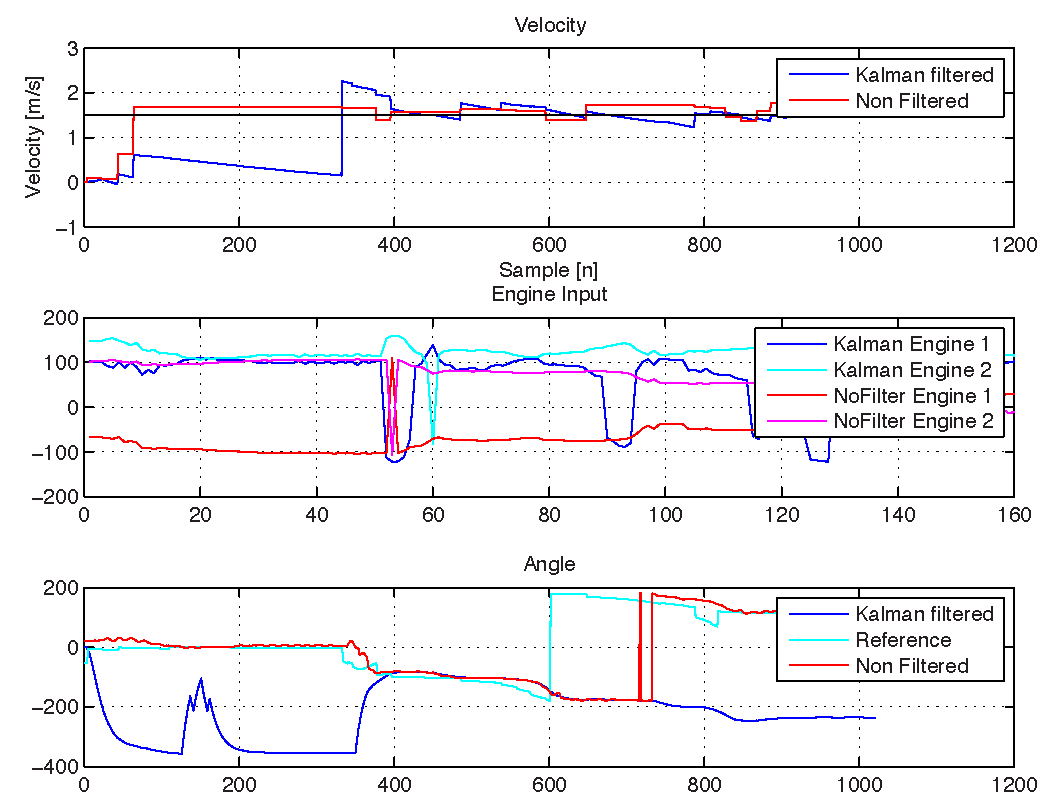
\includegraphics[width=8.4cm]{img/states}    % The printed column  
		\caption{Different states the system produces when sailing along the track depicted on figure \ref{fig:position}. As seen the system running on the non filtered data gives a wrong response as the ship would sail in circles at the start.}  % width of a column is 8.4 cm.
		\label{fig:states}               
	\end{center}                                 % accordingly.
\end{figure}

\subsection{System verification}
To ensure that the track sailed on figure \ref{fig:position} was not just a one of, the system was run multiple times with the same track as a reference. This produced as shown on figure \ref{fig:position2}. On the figure it is clearly seen that the ship consistently follows the contours of the track, but the estimates sometimes wander of due to loss of GPS reception.
\begin{figure}
	\begin{center}
		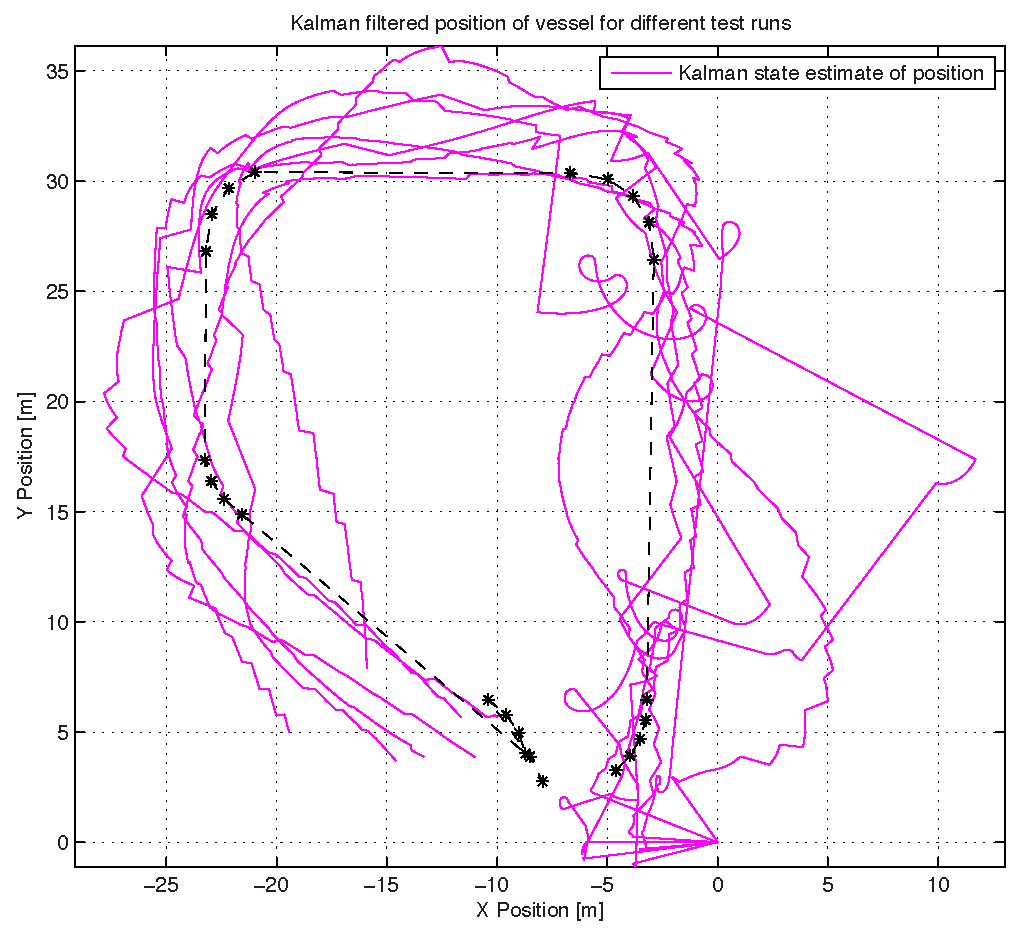
\includegraphics[width=8.4cm]{img/position2}    % The printed column  
		\caption{System verification with multiple tests run and plotted on top of the track. As seen the ship consistently follows the contours of the track, whilst at some points loosing some precision (due to bad GPS reception).}  % width of a column is 8.4 cm.
		\label{fig:position2}               
	\end{center}                                 % accordingly.
\end{figure}

\subsection{Errors}
As seen on figure \ref{fig:position2} the estimates wander off when the ship navigates in areas of bad GPS reception, this is due to the nonlinearity of the IMU, and the Kalman filter implemented being linear. 
\begin{figure}
	\begin{center}
		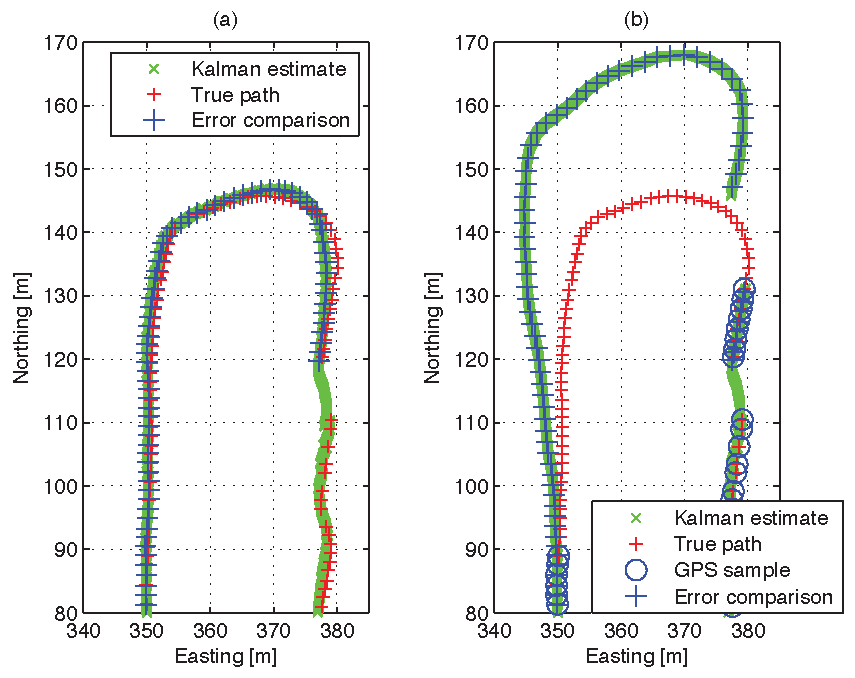
\includegraphics[width=8.4cm]{img/states2}    % The printed column  
		\caption{Kalman filtering, plot of the absolute position error. (a) depicts the error when the GPS is online at all times. (b) is when the GPS is offline for 60 seconds.}  % width of a column is 8.4 cm.
		\label{fig:states2}               
	\end{center}                                 % accordingly.
\end{figure}


\subsection{Discussion}
To further improve on the system, the Kalman filter should be extended to allow for the acceleration data also to be included in the position estimates, thus increasing the precision further when the GPS is offline. To make this feasible the bias of the IMU should be included in the model. Another feature of the Kalman filter would be to estimate the wind and current bias, which would cause the ship to veer off course. 

Throughout the tests the IMU have been assumed to always be level, which is hard to realize, so a slight bias is added, and with a linear Kalman filter which is hard compensate for as the IMU needs to always have the same bias for this to work. .

\section{Conclusion}
To sum up the project, a state estimator have been developed to improve on the GPS estimates allowing for a better precision if the GPS is offline. To plan the path the ship is to traverse a path planner have also been implemented showing good results. 

A final test of the combined system have not been conducted, as the waters around Aalborg have been frozen solid. 

\begin{ack}                               % Place acknowledgements
A special thank should be given to Assistant Professor Carles Navarro Manchòn, Section for Navigation and Communication, Department of Electronic Systems, Aalborg University for his help with tuning the Kalman filter and to School of Information and Communication Technlogy for the donation without which this project would not have succeder.  % here.
\end{ack}

%\bibliographystyle{alpha}        % Include this if you use bibtex 
%\bibliography{autosam}           % and a bib file to produce the 
%\bibliography{autosam}
                                 % bibliography (preferred). The
                                 % correct style is generated by
                                 % Elsevier at the time of printing.

\begin{thebibliography}{xx}

\bibitem[Ingeni\o ren(2012)]{engineer}
Birgitte Marfelt,
\newblock Ingeni\o ren
\newblock \emph{Tom pengekasse bremser søkort omkring Gr\o nland}
\newblock Mediehuset Ingeniøren, 2012

\bibitem[S\o rensen(2005)]{cyber}
Asgeir J. S\o rensen,
\newblock \emph{Marine Cybernetics, Modelling and Control - Lecture Notes}
\newblock Department of Marine Cybernetics, Norwegian University of Science and Technology, 2005

\bibitem[Franklin et. al.(2009)]{feedback}
Gene F. Franklin, J. David Powell and Abbas Emami-Naeini,
\newblock \emph{Feedback Control of Dynamic Systems, 5th ed.}
\newblock Pearson Prentice Hall, 2009

\bibitem[Department of Energy(2012)]{energy}
U.S. Department of Energy,
\newblock \emph{Radiological Assesment or effects from Fukushim Daiichi Nuclear Power Plant}
\newblock U.S. Department of Energy

\bibitem[Defense Update(2005)]{defense}
Defense Update, 2005, Issue 2,
\newblock \emph{Stingray, Unmanned Surface Vehcile (USV), Elbit Systems}
\newblock Defense Update

\end{thebibliography}
\end{document}
